Each sTGC trigger processor FPGA receives 32 fibers from the Routers on the rim of the NSW:
four fibers from each layer of the sTGC (each Router serves one layer).\footnote{Note that previously three fibers per layer were planned.}
With four input fibers per layer, up to four independent track segments can be calculated in four independent segment processors in the trigger processor FPGA.
The input links are FPGA-to-FPGA where the Router Xilinx Artix FPGA has GTP serializers whose maximum speed is $\approx$6.4\,Gb/s.
The trigger processor FPGA is a Xilinx Virtex\,7 which has GTH serializers whose maximum speed is in excess of 10\,Gb/s.
The input links to the Router from the Trigger Data Serializer ASICS run at 4.8\,Gb/s.
Using a higher output speed for the Router will allow use of 66b/64b or 8b/10b encoding to provide unambiguous framing.
(The input to the Router has unambiguous framing due to, for example, the 120b/116b encoding of the input packet, with one packet per BC.)
Three possible data formats are being considered that will allow the transfer of 6-bit ADC values from 14 or 15 strips, along with low bits of the BCID, the band ID, the $\phi$-id
and a flag indicating whether the high 15(14) of the 17 strips of a band or the low 15(14) strips are being transmitted.
The three possible formats for the data transmission from the strip-TDS to the Router are shown in Table\,\ref{tab:stripTDSout}.
In each bunch crossing, a packet is transmitted with a fixed header and a scrambled data payload.
Based on the null/data indicator, the Router either discards the packet or passes it to an available output fiber for transmission to the trigger processor.
Option\,1 requires the full 120-bit packet to be captured in order for the Router's descrambler to lock on the header.
The other options require only the first 30-bit packet to be captured for the routing decision and so has lower latency.
It is not yet clear if option\,1, with a 2-bit header, allows for reliable locking.

% Table generated by Excel2LaTeX from sheet 'Sheet1'
\begin{table}[htbp]
  \centering
  \small
    \tabcolsep=0.11cm
    \begin{tabular}{llrrrrrrrrrrrr}
    \toprule
    \multicolumn{2}{c}{\textbf{option}} & \textbf{strips} &       & \multicolumn{1}{c}{\textbf{hdr}} & \multicolumn{1}{c}{\textbf{flag}} & \multicolumn{6}{c}{\textbf{ field lengths (bits)}} & \multicolumn{1}{c}{\textbf{total}} & \multicolumn{1}{c}{\textbf{data}} \\
    \midrule
%          & five 30-bit & \multicolumn{1}{c}{15} &       & \multicolumn{1}{c}{20} & \multicolumn{1}{c}{10} & \multicolumn{1}{c}{8} & \multicolumn{1}{c}{1} & \multicolumn{1}{c}{90} & \multicolumn{1}{c}{5} & \multicolumn{1}{c}{12} & \multicolumn{1}{c}{4} & \multicolumn{1}{c}{\textbf{150}} & \multicolumn{1}{c}{120} \\
%    0     & packets with  &       & data  & \multicolumn{1}{c}{1010} & \multicolumn{1}{c}{10} & \multicolumn{1}{c}{band id} & \multicolumn{1}{c}{hi/lo} & \multicolumn{1}{c}{strips} & \multicolumn{1}{c}{$\phi$-id} & \multicolumn{1}{c}{\textsc{bcid}} & \multicolumn{1}{c}{\textsc{crc}} & \multicolumn{1}{c}{\textbf{}} & \multicolumn{1}{c}{} \\
%          & 2-bit header & \multicolumn{1}{c}{} & null  & \multicolumn{1}{c}{1010} & \multicolumn{1}{c}{01} & \multicolumn{1}{c}{} & \multicolumn{1}{c}{} & \multicolumn{1}{c}{} & \multicolumn{1}{c}{} & \multicolumn{1}{c}{} & \multicolumn{1}{c}{} & \multicolumn{1}{c}{} & \multicolumn{1}{c}{} \\
          & one 120-bit & \multicolumn{1}{c}{15} & \multicolumn{1}{l}{} & \multicolumn{1}{c}{4} & \multicolumn{1}{c}{0} & \multicolumn{1}{c}{8} & \multicolumn{1}{c}{1} & \multicolumn{1}{c}{90} & \multicolumn{1}{c}{5} & \multicolumn{1}{c}{12} & \multicolumn{1}{c}{0} & \multicolumn{1}{c}{\textbf{120}} & \multicolumn{1}{c}{116} \\
    1     & packet & \multicolumn{1}{c}{} & data  & \multicolumn{1}{c}{1010} & \multicolumn{1}{c}{} & \multicolumn{1}{c}{band id} & \multicolumn{1}{c}{hi/lo} & \multicolumn{1}{c}{strips} & \multicolumn{1}{c}{$\phi$-id} & \multicolumn{1}{c}{\textsc{bcid}} & \multicolumn{1}{c}{\textsc{crc}} & \multicolumn{1}{c}{\textbf{}} & \multicolumn{1}{c}{} \\
          &       &       & null  & \multicolumn{1}{c}{1100} & \multicolumn{1}{c}{} & \multicolumn{1}{c}{} & \multicolumn{1}{c}{} & \multicolumn{1}{c}{} & \multicolumn{1}{c}{} & \multicolumn{1}{c}{} & \multicolumn{1}{c}{} & \multicolumn{1}{c}{} & \multicolumn{1}{c}{} \\
          & \multicolumn{1}{l}{} & \multicolumn{1}{c}{} &       &       &       &       &       &       &       &       &       &       & \multicolumn{1}{c}{} \\
          & four 30-bit & \multicolumn{1}{c}{15} &       & \multicolumn{1}{c}{8} & \multicolumn{1}{c}{0} & \multicolumn{1}{c}{8} & \multicolumn{1}{c}{1} & \multicolumn{1}{c}{90} & \multicolumn{1}{c}{5} & \multicolumn{1}{c}{8} & \multicolumn{1}{c}{0} & \multicolumn{1}{c}{\textbf{120}} & \multicolumn{1}{c}{112} \\
    2     & packets with & \multicolumn{1}{c}{} & data  & \multicolumn{1}{c}{10} & \multicolumn{1}{c}{} & \multicolumn{1}{c}{band id} & \multicolumn{1}{c}{hi/lo} & \multicolumn{1}{c}{strips} & \multicolumn{1}{c}{$\phi$-id} & \multicolumn{1}{c}{\textsc{bcid}} & \multicolumn{1}{c}{\textsc{crc}} & \multicolumn{1}{c}{\textbf{}} & \multicolumn{1}{c}{} \\
          & 2-bit header &       & null  & \multicolumn{1}{c}{01} & \multicolumn{1}{c}{} & \multicolumn{1}{c}{} & \multicolumn{1}{c}{} & \multicolumn{1}{c}{} & \multicolumn{1}{c}{} & \multicolumn{1}{c}{} & \multicolumn{1}{c}{} & \multicolumn{1}{c}{} & \multicolumn{1}{c}{} \\
          & \multicolumn{1}{l}{} & \multicolumn{1}{c}{} &       &       &       &       &       &       &       &       &       &       & \multicolumn{1}{c}{} \\
          & four 30-bit & \multicolumn{1}{c}{14} &       & \multicolumn{1}{c}{16} & \multicolumn{1}{c}{0} & \multicolumn{1}{c}{8} & \multicolumn{1}{c}{1} & \multicolumn{1}{c}{84} & \multicolumn{1}{c}{5} & \multicolumn{1}{c}{6} & \multicolumn{1}{c}{0} & \multicolumn{1}{c}{\textbf{120}} & \multicolumn{1}{c}{104} \\
    3     & packets with &       & data  & \multicolumn{1}{c}{1010} & \multicolumn{1}{c}{} & \multicolumn{1}{c}{band id} & \multicolumn{1}{c}{hi/lo} & \multicolumn{1}{c}{strips} & \multicolumn{1}{c}{$\phi$-id} & \multicolumn{1}{c}{\textsc{bcid}} & \multicolumn{1}{c}{\textsc{crc}} &       &  \\
          & 4-bit header & \multicolumn{1}{c}{} & null  & \multicolumn{1}{c}{1100} & \multicolumn{1}{c}{} & \multicolumn{1}{c}{} & \multicolumn{1}{c}{} & \multicolumn{1}{c}{} & \multicolumn{1}{c}{} & \multicolumn{1}{c}{} & \multicolumn{1}{c}{} & \multicolumn{1}{c}{} &  \\
    \bottomrule
    \end{tabular}%
   \caption{Options for data formats for the data transmission from the strip-TDS to the Router.}
   \label{tab:stripTDSout}%
\end{table}%

%After descrambling, the Router will recode the data in 8b/10 code with a comma character between bunch crossings.
Options~1,~2 and~3 require 6.4\,Gb/s and 6.0\,Gb/s and 5.6\,Gb/s rates, respectively, in order to send 8b/10b encoded data within 25\,ns.
The 64b/66b encoding requires 5.28~Gb/s, but may have slightly longer latency.
The Router's Artix FPGA's (upper limit is 6.6\,Gb/s) and opto-electronics allow these speeds.

\paragraph{Preparation of the input to the sTGC algorithm}  \hfill \\

A complication arises from the fact that strip bands may span two TDS ASICs. In this case each TDS ASIC transmits the strip data that it has.
The Router then receives two active inputs for a single candidate.
For simplicity and to reduce latency, the Router does not merge the two streams to a single output fiber, but just passes them on to two fibers.
The trigger processor then must route the input bits to their correct location in the 17-strip input word for the centroid finders.
A further complication, due to the pointing geometry, is that a band that spans two TDS ASICs in one layer may be fully contained in a single TDS in another layer.
The input processor must take this into account and route all the data of all layers to the same segment processor.
Alternatively, the centroids in each layer could be routed after they are found, but before they are input to the segment calculator block.

The various input links will not have the same phase and may not even be matched to the same BC clock. The input processor must ensure that all sources are aligned to the same BC clock.

%%%%%%%%% Sample inclusion of a figure
 % \begin{figure}[h]
 % \begin{center}
 % 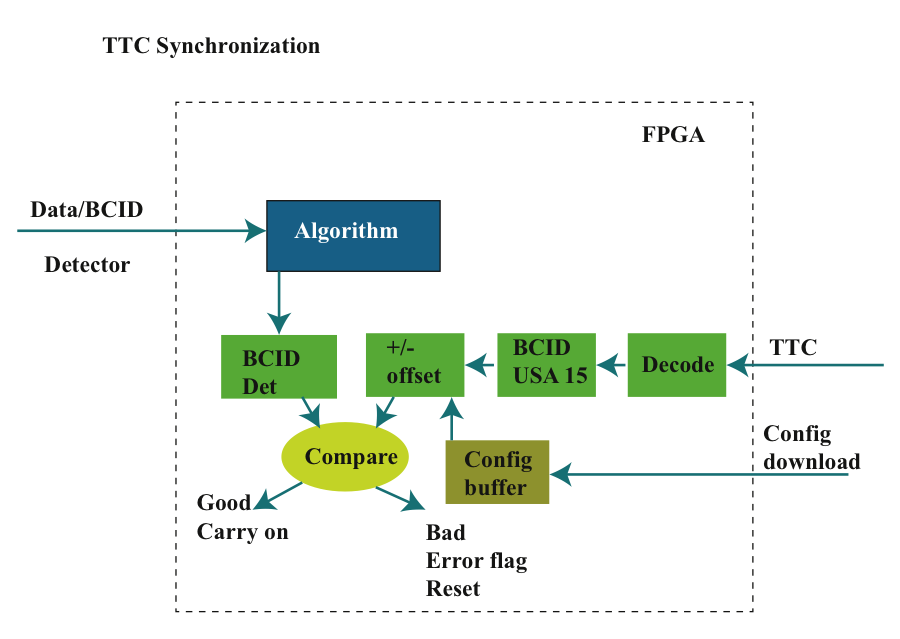
\includegraphics[width=0.8\textwidth]{specs/Diagram-TTCSync}
 % \caption{Block diagram of an implementation of the TTC synchronization.}
 % \label{fig:Monitoring}
 % \end{center}
 % \end{figure}
